\documentclass[conference]{IEEEtran}

\IEEEoverridecommandlockouts

\usepackage[T1]{fontenc}
\usepackage{cite}
\usepackage{amsmath,amssymb}
\usepackage{booktabs}
\usepackage{graphicx}
\usepackage{array}
\usepackage{tabularx}
\usepackage{multirow}
\usepackage{xcolor}
\usepackage{url}
\usepackage{balance}

\newcolumntype{Y}{>{\raggedright\arraybackslash}X}

\definecolor{magmaNavy}{HTML}{14213D}
\definecolor{magmaBlue}{HTML}{1D4E89}
\definecolor{magmaTeal}{HTML}{14919B}
\definecolor{magmaOrange}{HTML}{F39C12}
\definecolor{magmaPink}{HTML}{C2185B}
\definecolor{magmaGreen}{HTML}{2A9D55}
\definecolor{magmaGray}{HTML}{5D6673}

\newcommand{\toolone}{T1}
\newcommand{\tooltwo}{T2}
\newcommand{\magma}{\textsc{Magma}}

\title{\magma: Hybrid FFF-Printed Mold Injection on a Multi-Tool Desktop Printer}

\author{
\IEEEauthorblockN{Ethan Childerhose}
\IEEEauthorblockA{
Bracket Bot Research \\
San Francisco, CA, USA \\
June 2026 internal research draft}
}

\begin{document}
\maketitle

\begin{abstract}
This paper presents \magma, an experimental hybrid manufacturing workflow in which a desktop multi-tool fused filament fabrication (FFF) printer first fabricates a thermoplastic mold and then uses a second heated tool as a low-pressure melt delivery system. The near-term platform is a Prusa XL-style printer configured with a PETG mold tool and a larger PLA injection nozzle. Unlike approaches that reinforce sparse infill, the target part is represented as a separate molded volume: the slicer or post-processor suppresses that body from normal printing, computes its volume, locates an injection port, and emits a controlled tool-change, heating, and extrusion sequence. Early trials show that injected melt can be delivered into printed cavities, but reliable filling depends on port geometry, thermal management, volumetric flow rate, tool pickup sequencing, and collision-safe nozzle motion. We describe the system concept, a role-based CAD-to-G-code workflow, a first experimental protocol, and the software path from a G-code post-processor toward native slicer support.
\end{abstract}

\begin{IEEEkeywords}
additive manufacturing, fused filament fabrication, injection molding, multi-material printing, slicer software, desktop manufacturing
\end{IEEEkeywords}

\section{Introduction}
Fused filament fabrication is effective for rapid iteration because it turns a digital model into a physical object without dedicated tooling. However, FFF parts inherit the limitations of layer-wise bead deposition, including anisotropic interlayer bonding, visible toolpaths, and material flow histories that differ substantially from molded plastic. Injection molding, by contrast, can produce dense thermoplastic parts with continuous melt flow and good surface finish, but it typically requires rigid tooling, clamping, and a dedicated press.

This work investigates an intermediate process: using the printer itself to fabricate a mold, then using another printer toolhead to fill that mold with molten thermoplastic. The immediate goal is not to reproduce industrial injection molding pressure or packing. Instead, the project asks whether a multi-tool FFF platform can support a repeatable, low-pressure molded deposition workflow for small cavities. If the process can be made reliable, it would enable fast iteration on mold geometry, port placement, material pairing, and process control without moving to a separate molding machine.

The project is motivated by a practical hardware opportunity. Modern tool-changing FFF printers can park multiple heated extruders and select them under G-code control. A smaller nozzle can print accurate mold features, while a larger nozzle can act as a melt delivery tool. The same machine can therefore run a two-stage process: print the tool, then inject the part.

\begin{figure}[t]
\centering
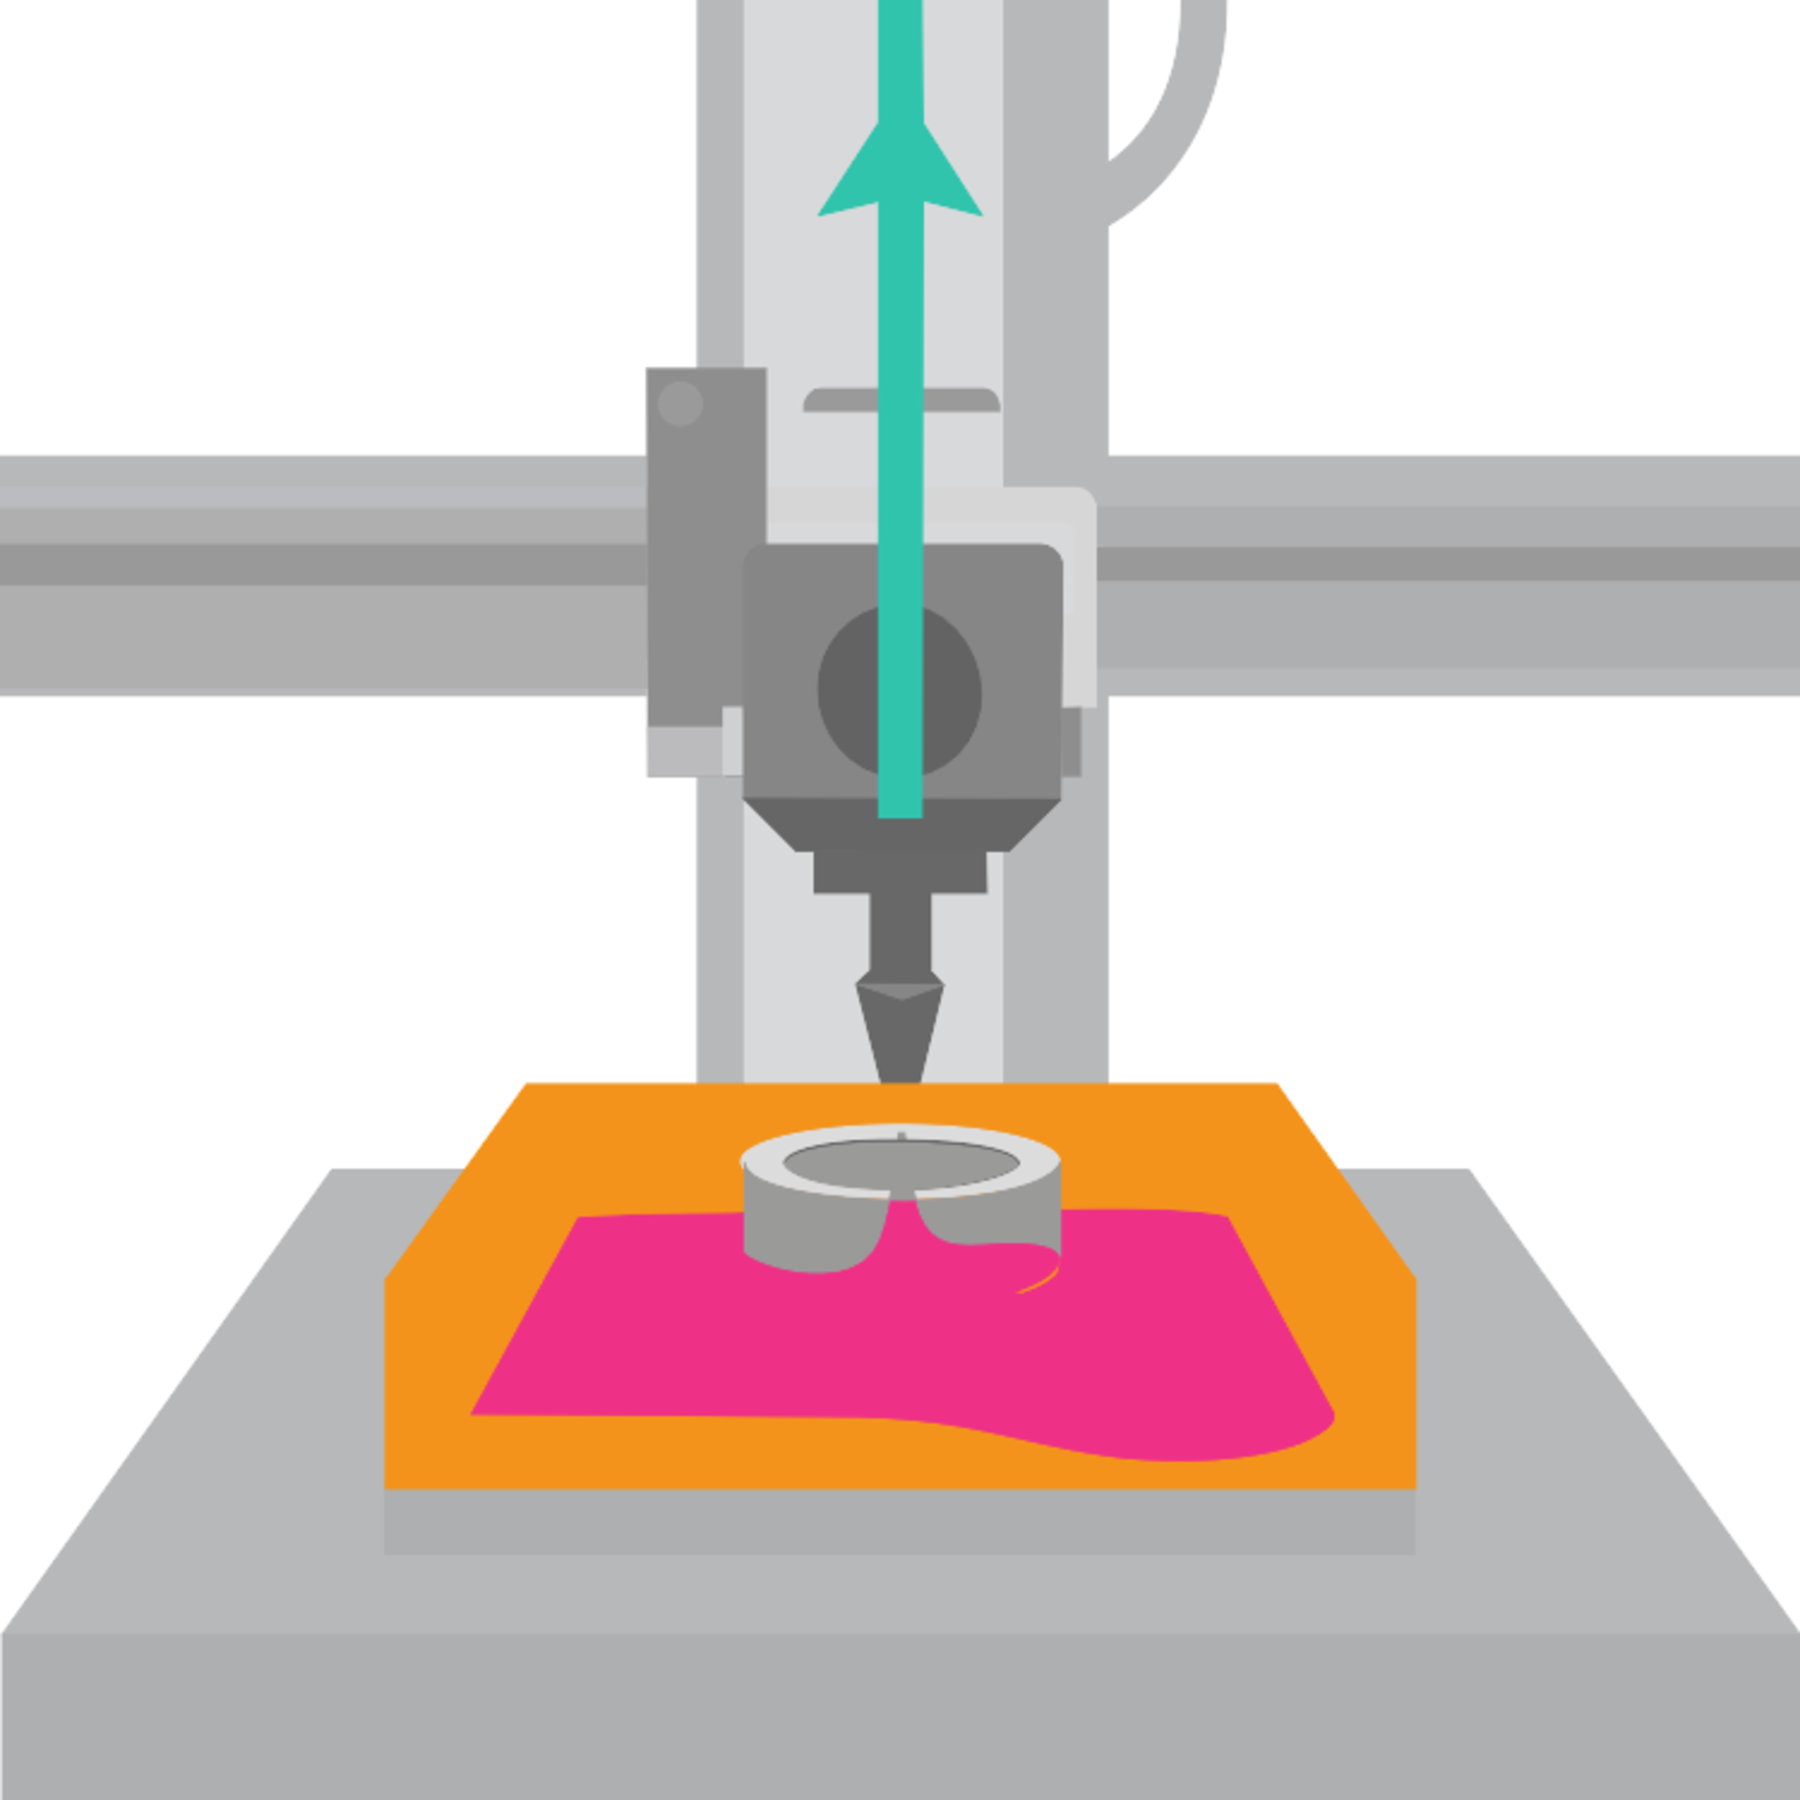
\includegraphics[width=\columnwidth]{figures/quiver_system_concept.png}
\caption{QuiverAI-generated conceptual process figure. A first tool prints a PETG mold, while a second larger nozzle injects PLA through a port. Later versions can begin closer to the cavity floor and rise during filling.}
\label{fig:concept}
\end{figure}

\section{Process Concept}
The \magma\ workflow treats the printer as a programmable thermal material delivery system. During the mold stage, conventional FFF slicing produces the walls, floor, split mold bodies, or test cup. During the injection stage, the printer selects the injection tool, raises it to the requested temperature, moves to the injection port, and extrudes a calculated volume of melt.

The initial experiments are intentionally simple. A 10 mm-scale open cavity can be printed quickly, filled with little material, and inspected immediately. This establishes whether the hotend can deliver enough molten polymer before the material freezes against the mold walls. The current working material pair is PETG for the mold and PLA for the injected material. PETG is used because it provides more thermal margin than PLA for a printed mold, while PLA is used for early injection because it melts at relatively accessible temperatures and extrudes reliably.

The process differs from conventional injection molding in pressure, stiffness, and thermal boundary conditions. A desktop hotend cannot instantly melt arbitrary flow rates, and the printed mold can soften, leak, or block if the port is poorly designed. The appropriate first framing is therefore low-pressure molded deposition into additively manufactured tooling.

\section{Role-Based CAD and Slicer Workflow}
The desired CAD workflow uses distinct model roles rather than a single printable mesh. The mold bodies are printed. The injected part body is not printed directly; instead, it defines the volume to be filled. A port marker identifies the intended injection location, and optional vent or overflow bodies can define escape paths.

\begin{figure*}[t]
\centering

\includegraphics[width=0.92\textwidth]{figures/quiver_slicer_pipeline.png}
\caption{QuiverAI-generated software-pipeline figure. The intended stages are named CAD bodies, role classification, volume solving, and G-code emission. Named STEP bodies allow the slicer to classify printable mold geometry separately from the injected volume and injection port.}
\label{fig:pipeline}
\end{figure*}

Fig.~\ref{fig:pipeline} shows the target software pipeline. The most important behavior is suppressing helper bodies from ordinary FFF toolpath generation. If the injection port marker is treated as a normal solid, the slicer may close or block the port, making the preview misleading and the mold impossible to fill. Likewise, if the injected part body is printed as normal geometry, the process is no longer injection into a mold.

The injected filament length should be related to the desired part volume. For filament diameter $d_f$ and target injected volume $V_i$, the ideal commanded extrusion length is
\begin{equation}
E = \frac{4 V_i}{\pi d_f^2}.
\label{eq:extrusion}
\end{equation}
A multiplier can compensate for leakage, shrinkage, port dead volume, or intentional overfill. The slicer should also chunk extrusion into firmware-safe moves and check that the requested volumetric flow rate does not exceed the hotend's practical melting capacity.

\section{Current Software Prototype}
The current fast-learning implementation is a post-processor rather than a fully native slicer feature. The local prototype, \texttt{magma\_inject.py}, takes sliced mold G-code, detects or receives a cavity volume, and splices an injection sequence before the print end code. It can rasterize extruded G-code paths and flood-fill enclosed empty regions to estimate the cavity location, or use STL geometry to detect a pocket. It then estimates the injection XY coordinate, selects the injection tool, heats it, and emits a controlled extrusion block.

This post-processing path is useful because it separates process learning from slicer UI work. Parameters such as temperature, injection tool, fill fraction, plunge depth, volume override, and volumetric flow rate can be changed quickly between prints. However, a G-code post-processor is brittle for general users: it depends on coordinate assumptions, tool-change details, and preview conventions that are not explicit in the slicer. Native support is required for a production-quality workflow.

\section{Experimental Method}
The experimental plan is to start with a geometry that is too simple to hide the failure mode. A small cup, cylinder, or cube-shaped cavity should be printed in PETG. The injection port must be a real opening into the cavity, not a decorative or printed solid placed on top. The PLA injection tool is heated above ordinary print temperature if needed to lower viscosity and increase delivered melt.

\begin{table}[t]
\caption{Initial Experimental Configuration}
\label{tab:config}
\centering
\scriptsize
\setlength{\tabcolsep}{2.4pt}
\begin{tabularx}{\columnwidth}{@{}p{0.27\columnwidth}p{0.29\columnwidth}Y@{}}
\toprule
Parameter & Current value & Purpose \\
\midrule
Mold tool/material & \toolone, 0.4 mm, PETG & Accurate cavity and thermal margin \\
Injection tool/material & \tooltwo, 0.8 mm, PLA & Larger melt outlet and lower melt temperature \\
Initial geometry & 10 mm cup/cube & Fast iteration and low material risk \\
Injection command & Part/cavity volume & Match extrusion to molded volume \\
Near-term sweep & 240--275 C, 10--30 mm$^3$/s & Map the fill window before complex molds \\
\bottomrule
\end{tabularx}
\end{table}

\begin{figure}[t]
\centering

\includegraphics[width=\columnwidth]{figures/quiver_model_roles.png}
\caption{QuiverAI-generated role-modeling figure. The design should contain printable mold bodies, a non-printing injected part body, and a non-printing injection-port marker.}
\label{fig:roles}
\end{figure}

Table~\ref{tab:config} summarizes the first test configuration. The print sequence is:
\begin{enumerate}
\item print the mold using the mold tool and mold material;
\item heat, pick, and optionally purge the injection tool;
\item move to the injection port at a collision-safe approach height;
\item extrude the computed volume at a controlled volumetric flow rate;
\item inspect fill depth, leakage, port blockage, mold deformation, stringing, and removal quality.
\end{enumerate}

Early observations suggest that top-only injection can underfill the bottom of a cavity if the melt cools before it reaches the floor. The proposed rising-Z schedule begins near the lower cavity region, extrudes while the melt front grows, then rises as the fill level increases. This must be combined with collision checking, because multi-tool printer geometry can make downward approaches unsafe near tall mold walls.

\section{Preliminary Observations}
The initial development work produced several useful observations. First, the printer can be driven by custom G-code that prints a small mold-like geometry and then executes an injection sequence. Second, molten plastic delivery into a printed cavity is possible. Third, process reliability is sensitive to temperature, flow, and port geometry. If extrusion is commanded too quickly, the hotend may not melt filament fast enough or firmware limits may reduce the delivered volume. If extrusion is too slow, the melt can lose heat and freeze against the mold before the lower cavity is filled.

The team also observed that tool-change and parked-tool behavior matter. A tool parked at a lower standby temperature may not be ready when the printer picks it up unless the G-code explicitly waits for the target injection temperature. Purging and nozzle cleaning are also relevant because material on the nozzle can interfere with port seating or contaminate the mold. These are ordinary printer concerns, but they become process-critical when the nozzle is used as an injection element.

\begin{figure}[t]
\centering

\includegraphics[width=\columnwidth]{figures/quiver_process_window.png}
\caption{QuiverAI-generated process-window figure. Reliable filling requires enough heat and flow to reach the bottom of the cavity without exceeding hotend melting capacity or deforming the mold. The intended axes are volumetric flow rate and injection temperature.}
\label{fig:window}
\end{figure}

Fig.~\ref{fig:window} summarizes the expected process window. The most important failure labels for the next dataset are underfill, blocked port, leakage, mold softening, and unmelted or firmware-limited extrusion.

\section{Roadmap to Native Slicer Support}
The development roadmap has four stages. Phase 0 is the current G-code post-processing path for simple open cavities and manual parameter sweeps. Phase 1 adds native slicer settings for injection volume, port location, tool selection, temperature, and preview. Phase 2 imports named STEP bodies and validates that mold, injected part, and port roles are geometrically consistent. Phase 3 adds rising-Z fill paths, vents, overflow reservoirs, and collision checking. Phase 4 compares mechanical and dimensional results against conventional FFF prints of the same part.

\begin{table}[t]
\caption{Validation Matrix for the First Paper-Quality Dataset}
\label{tab:validation}
\centering
\scriptsize
\setlength{\tabcolsep}{2.2pt}
\begin{tabularx}{\columnwidth}{@{}p{0.24\columnwidth}p{0.23\columnwidth}p{0.25\columnwidth}Y@{}}
\toprule
Variable & Sweep & Primary metric & Failure label \\
\midrule
Nozzle temperature & 240, 255, 275 C & Bottom fill depth & Freezing \\
Flow rate & 10, 20, 30 mm$^3$/s & Delivered mass & Flow limit \\
Port geometry & Diameter, chamfer & Leakage/blockage & Port failure \\
Z schedule & Top pour, rising-Z & Void fraction & Trapped air \\
\bottomrule
\end{tabularx}
\end{table}

Table~\ref{tab:validation} gives the first dataset that should be collected for a publication-quality revision. The dataset should remain deliberately simple. A 10 mm cavity with a real top port is enough to determine whether changes in temperature, flow, port design, and Z schedule improve fill completeness. More complex Benchy-derived or application-specific molds should wait until the simple dataset is interpretable.

\section{Discussion}
\magma\ is promising because it uses hardware that already exists on multi-tool FFF printers. The printer can fabricate disposable tooling, hold multiple materials, change tools under G-code control, and position the injection nozzle repeatably relative to the printed mold. This makes the approach attractive for rapid mold iteration and low-volume experimental parts.

The same integration creates risks. Slicer previews are normally path-centric, but the injected volume is not a normal printed path. A credible user interface must show the mold, the non-printing injected part body, the port, vents, overflow regions, and the planned injection move. It should also warn when the port is blocked, when the injected body does not intersect the cavity, or when the requested flow rate is outside the tool's plausible melt capacity.

The project should avoid overclaiming. Current experiments are pour-like and do not create industrial packing pressure. Tall, thin, or poorly vented cavities may fail. The mold material may soften or bond to the injected material. These limitations do not invalidate the workflow; they define the first engineering problems the slicer and process need to solve.

\section{Limitations and Safety}
The present process should be treated as an exploratory manufacturing mode, not as a drop-in substitute for a press. The printer has no clamp force, no pressure sensor at the melt front, and no direct observation of the cavity once the mold is closed. A failed fill can therefore look like a successful extrusion command unless the experiment records mass, visual fill depth, or a sectioned part.

Thermal safety also matters. The injection nozzle may be run hotter than normal PLA printing in order to improve flow, while the PETG mold remains close to the melt source for an extended time. The software should prevent accidental contact between the injection nozzle and printed walls, enforce a safe dwell limit, and keep all injection moves inside a collision-checked envelope. Vents and overflow reservoirs should be designed intentionally so trapped air and excess material leave through known paths rather than splitting the mold or forcing material upward around the nozzle.

\section{Future Work}
The next experiments should prioritize interpretable data over complex shapes. A single 10 mm cavity with a known port diameter is sufficient to sweep temperature, volumetric flow, and Z schedule. Each trial should record the commanded volume, actual mass change, visible fill height, leakage, and whether the part reaches the mold floor. Once that dataset identifies a stable operating region, the same procedure can be repeated with split molds, more realistic port/vent layouts, and shaped cavities such as the Benchy-derived test mold.

On the software side, the most important addition is a validation pass before slicing. The slicer should verify that the injected body is inside the mold cavity, the port connects to the cavity, and the selected tool can physically approach the port without colliding with printed geometry. A dedicated preview should show the mold as transparent or sectioned, overlay the injected volume, and display the exact injection move sequence separately from normal extrusion paths.

\section{Conclusion}
This paper introduced \magma, a hybrid desktop manufacturing workflow that combines an FFF-printed mold with low-pressure thermoplastic injection from a second printer tool. The concept is strongest when the slicer understands three separate roles: the printable mold, the non-printing injected part volume, and the injection port. The current G-code post-processing path is sufficient for process discovery, while native slicer support is needed for repeatable geometry handling, preview, and safety. The next critical step is a clean experimental matrix that quantifies the fill window before scaling to complex molds.

\balance
\begin{thebibliography}{00}
\bibitem{iso52900}
ISO/ASTM 52900:2021, ``Additive manufacturing -- General principles -- Fundamentals and vocabulary,'' International Organization for Standardization, 2021.

\bibitem{prusaXL}
Prusa Research, ``Original Prusa XL,'' product and technical documentation. [Online]. Available: \url{https://www.prusa3d.com/product/original-prusa-xl-2/}

\bibitem{prusaslicer}
Prusa Research, ``PrusaSlicer,'' open-source repository. [Online]. Available: \url{https://github.com/prusa3d/PrusaSlicer}

\bibitem{orcaslicer}
SoftFever, ``OrcaSlicer,'' open-source repository. [Online]. Available: \url{https://github.com/SoftFever/OrcaSlicer}

\bibitem{magma}
E. Childerhose, ``Magma injection post-processor and multi-tool injection G-code trials,'' local prototype, June 2026.
\end{thebibliography}

\end{document}
